\documentclass[Main.tex]{subfiles}
\begin{document}

\section{Residual Plots}
	%http://blog.minitab.com/blog/adventures-in-statistics/why-you-need-to-check-your-residual-plots-for-regression-analysis
	In the graph above, you can predict non-zero values for the residuals based on the fitted value. For example, a fitted value of 8 has an expected residual that is negative. Conversely, a fitted value of 5 or 11 has an expected residual that is positive.
	
	The non-random pattern in the residuals indicates that the deterministic portion (predictor variables) of the model is not capturing some explanatory information that is “leaking” into the residuals. The graph could represent several ways in which the model is not explaining all that is possible. 
	
	Possibilities include:
	
	\begin{itemize}
		\item A missing variable
		\item A missing higher-order term of a variable in the model to explain the curvature
		\item A missing interction between terms already in the model
	\end{itemize}
	
	
	Identifying and fixing the problem so that the predictors now explain the information that they missed before should produce a good-looking set of residuals.
	
	In addition to the above, here are two more specific ways that predictive information can sneak into the residuals:
	
	The residuals should not be correlated with another variable. If you can predict the residuals with another variable, that variable should be included in the model. In Minitab’s regression, you can plot the residuals by other variables to look for this problem.
	
	\noindent \textbf{Autocorrelation} \\
	Adjacent residuals should not be correlated with each other (\textbf{autocorrelation}). If you can use one residual to predict the next residual, there is some predictive information present that is not captured by the predictors. Typically, this situation involves time-ordered observations. For example, if a residual is more likely to be followed by another residual that has the same sign, adjacent residuals are positively correlated. You can include a variable that captures the relevant time-related information, or use a time series analysis. 
	
	In Minitab’s regression, you can perform the \textbf{\textit{Durbin-Watson} }test to test for autocorrelation.
	
	
	
	
	
	
	
	
	
	
	
	
%=================================================== %
% http://www.ime.usp.br/~jmsinger/MAE0610/Mixedmodelresiduals.pdf
\subsection{Residual Plots}
A residual plot is a graph that shows the residuals on the vertical axis and the independent variable on the horizontal axis. If the points in a residual plot are randomly dispersed around the horizontal axis, a linear regression model is appropriate for the data; otherwise, a non-linear model is more appropriate.

Below the table on the left shows inputs and outputs from a simple linear regression analysis, and the chart on the right displays the residual (e) and independent variable (X) as a residual plot.

%x	60	70	80	85	95
%y	70	65	70	95	85
%ŷ	65.411	71.849	78.288	81.507	87.945
%e	4.589	-6.849	-8.288	13.493	-2.945
% Image of residual plot

The residual plot shows a fairly random pattern - the first residual is positive, the next two are negative, the fourth is positive, and the last residual is negative. This random pattern indicates that a linear model provides a decent fit to the data.

Below, the residual plots show three typical patterns. The first plot shows a random pattern, indicating a good fit for a linear model. The other plot patterns are non-random (U-shaped and inverted U), suggesting a better fit for a non-linear model.


%Random pattern	Non-random: U-shaped	Non-random: Inverted U
In the next lesson, we will work on a problem, where the residual plot shows a non-random pattern. And we will show how to "transform" the data to use a linear model with nonlinear data.



\section{Diagnostic Plots for Linear Models with \texttt{R}}
Plot Diagnostics for an \texttt{lm} Object

%% \subsection{Description}

Six plots (selectable by \texttt{which}) are currently available: 
\begin{enumerate}
	\item a plot of residuals against fitted values, 
	\item a Scale-Location plot of \textit{sqrt(| residuals |}) against fitted values, 
	\item a Normal Q-Q plot, 
	\item a plot of Cook's distances versus row labels, 
	\item a plot of residuals against leverages, 
	\item a plot of Cook's distances against leverage/(1-leverage).
\end{enumerate} By default, the first three and 5 are provided.
%====================================================================%
\subsubsection{Residuals plots}

lme allows to plot the residuals in the following ways:

\begin{framed}
	\begin{verbatim}
	res_lme=residuals(model_lme)
	plot(res_lme)
	qqnorm(res_lme)
	qqline(res_lme)
	plot(model_lme)
	\end{verbatim}
\end{framed}

When the \texttt{plot} function calls the model object, the residual plot is produced.


%====================================================================%


\begin{framed}
	\begin{verbatim}
	plot(JS.roy1, which=c(1) )
	\end{verbatim}
\end{framed}

LME models assume that the residuals of the model are normally distributed. A Normal probability plot can be constructed to check this assumption. Commonly used \texttt{R} commands can be used to construct the plot.


\begin{framed}
	\begin{verbatim}
	qqnorm(resid(JS.roy1),pch="*",col="red")
	qqline(resid(JS.roy1),col="blue")
	\end{verbatim}
\end{framed}

\begin{framed}
	\begin{verbatim}
	table(dat$method[1:255])
	## 
	##   J   S 
	## 255   0
	table(dat$method[256:510])
	## 
	##   J   S 
	##   0 255
	\end{verbatim}	
\end{framed}
\begin{framed}
	\begin{verbatim}
	library(predictMeans)
	CookD(model, group=method, plot=TRUE, idn=5, newwd=FALSE)
	\end{verbatim}
\end{framed}






\begin{framed}
	\begin{verbatim}
	> shapiro.test(resid(JS.roy1)[256:510])
	
	Shapiro-Wilk normality test
	
	data:  resid(JS.roy1)[256:510]
	W = 0.9395, p-value = 9.503e-09
	\end{verbatim}
\end{framed}
%	\begin{figure}[h!]
%		\centering
%		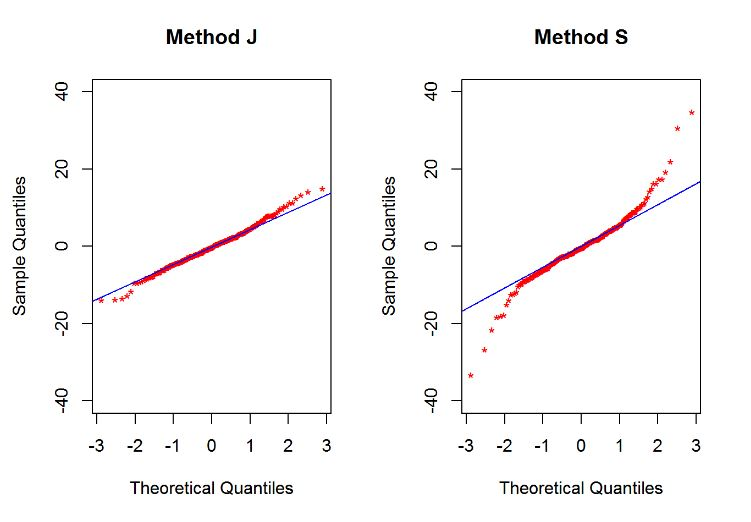
\includegraphics[width=0.9\linewidth]{images/Resid-newplot2}
%		
%	\end{figure}

\begin{framed}
	\begin{verbatim}
	plot(roy.NLME, resid(., type = "p") ~ fitted(.) | method, 
	abline = 0, id=.05)
	\end{verbatim}
\end{framed}
%	\begin{figure}
%		\centering
%		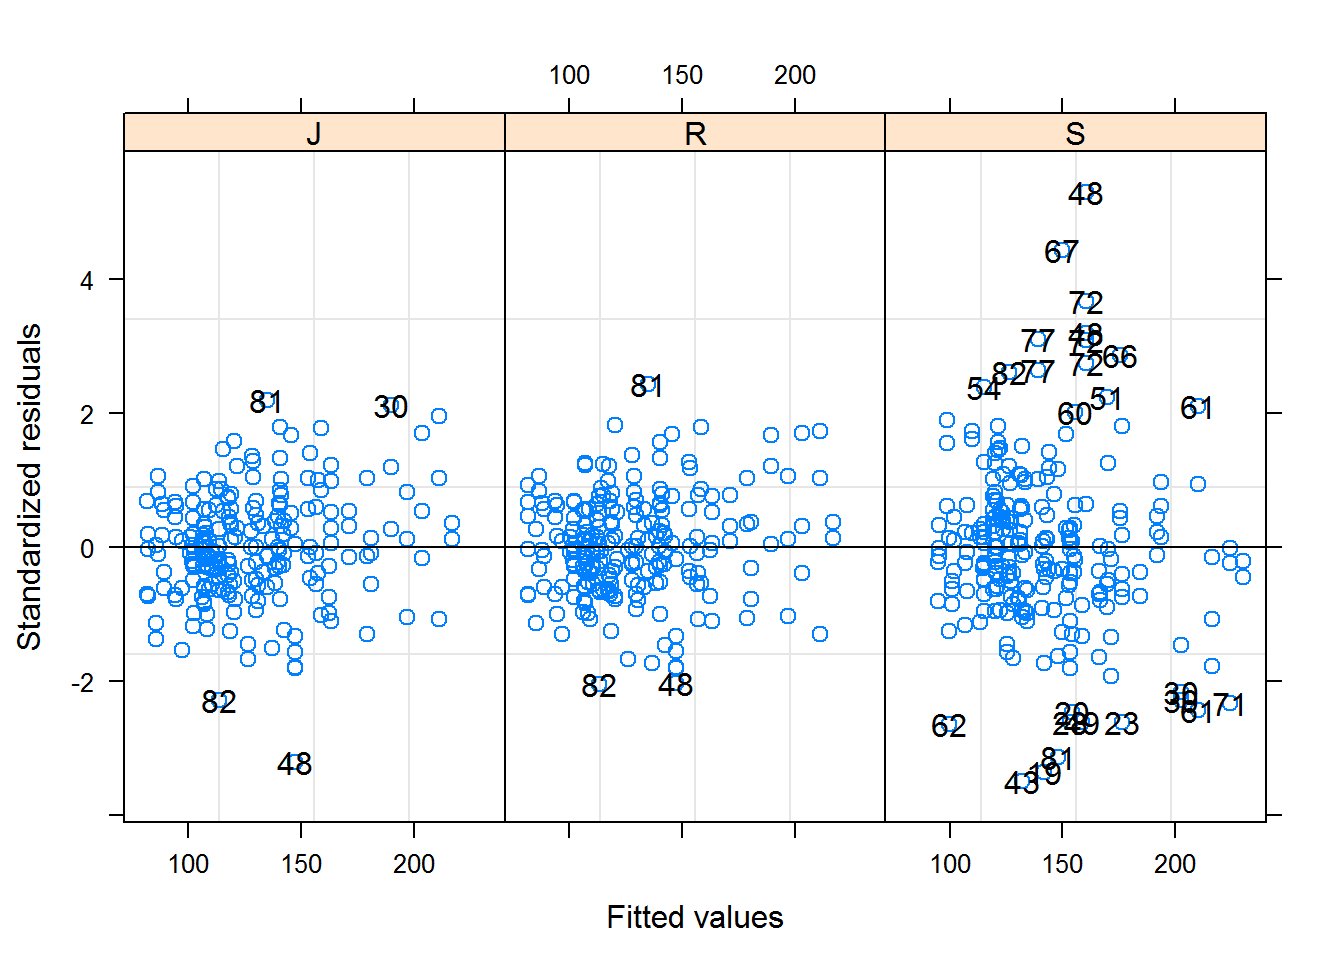
\includegraphics[width=0.9\linewidth]{images/bloodnlmeResidPlot2}
%		\caption{}
%		\label{fig:blood}
%	\end{figure}

\begin{framed}
	\begin{verbatim}
	library(predictMeans)
	CookD(model, group=method, plot=TRUE, idn=5, newwd=FALSE)
	\end{verbatim}
\end{framed}



\begin{framed}
	\begin{verbatim}
	
	blood.red <- blood[!(blood$subject %in% c(68,78,80)),]
	dim(blood.red)
	# 27 observations should be removed.
	
	blood.NLME.red <-lme(BP ~ method-1 , random=~1|subject,data = blood.red)
	plot(blood.NLME.red, resid(., type = "p") ~ fitted(.) | method, abline = 0, id=.05)
	\end{verbatim}
\end{framed}


\begin{framed}
	\begin{verbatim}
	> shapiro.test(resid(JS.roy1)[1:255])
	
	Shapiro-Wilk normality test
	
	data:  resid(JS.roy1)[1:255]
	W = 0.9931, p-value = 0.2852
	\end{verbatim}
\end{framed}

\begin{framed}
	\begin{verbatim}
	> shapiro.test(resid(JS.roy1)[256:510])
	
	Shapiro-Wilk normality test
	
	data:  resid(JS.roy1)[256:510]
	W = 0.9395, p-value = 9.503e-09
	\end{verbatim}
\end{framed}
%	\begin{figure}[h!]
%		\centering
%		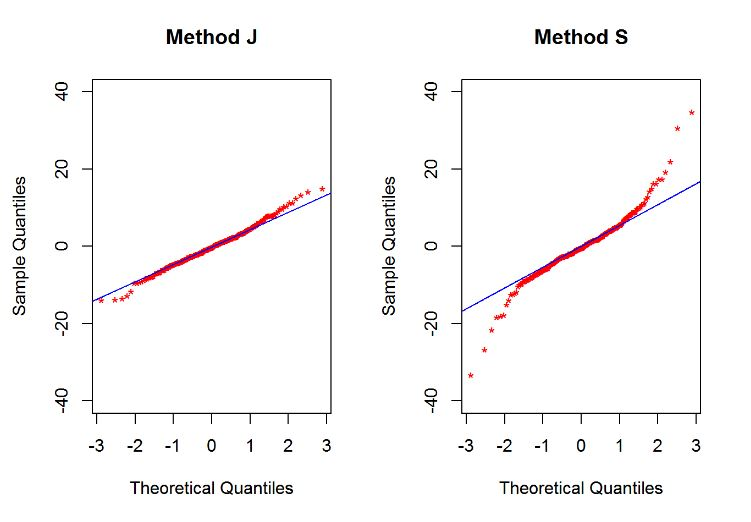
\includegraphics[width=0.9\linewidth]{images/Resid-newplot2}
%		
%	\end{figure}



\begin{framed}
	\begin{verbatim}
	data.frame( response = resid(JS.ARoy20091, type = "response"), 
	pearson  = resid(JS.ARoy20091, type = "pearson"), 
	normalized = resid(JS.ARoy20091, type = "normalized") )
	\end{verbatim}
\end{framed}

\begin{verbatim}
response      pearson    normalized
1    -4.65805902 -0.761587227 -0.7615872269
2    -0.88701342 -0.145025661  0.0776238081
3    -5.16580898 -0.844603753 -0.8446037530
4     2.29041830  0.374480726  0.6450898404
5     7.87508366  1.287567009  1.2875670086
6    -6.57048659 -1.074266908 -1.5090772378
...........................................
\end{verbatim}
For the $J$ observations, the variance is 6.116252 whereas for the $S$ observations, the denominator is 9.118144. (with the expected ratio of  1.490806)


\begin{framed}
	\begin{verbatim}
	> pearson %>%
	+   as.numeric %>% 
	+   matrix(nrow=85) %>%
	+   round(4) 
	[,1]    [,2]    [,3]    [,4]    [,5]    [,6]
	[1,] -0.7616  0.2194  0.3829 -0.2983  0.3597 -0.0790
	[2,] -0.1450  0.1820 -0.1450 -0.5014  0.1567  0.2663
	[3,] -0.8446  0.4634  0.1364 -0.1630 -0.2727  0.1660
	[4,]  0.3745 -0.2795 -0.2795 -0.2658 -0.2658  0.6115
	[5,]  1.2876 -0.6744 -0.6744  0.8935 -0.0935 -0.8612
	[6,] -1.0743  1.8687 -0.7473 -0.0383  0.2908 -0.3673
	...........................................
	
	\end{verbatim}
\end{framed}

We can plot the residuals against the fitted values, to assess the assumption of constant variance. 
\begin{framed}
	\begin{verbatim}
	# standardized residuals versus fitted values 
	plot(JS.ARoy20091, resid(., type = "pearson") ~ fitted(.) , 
	abline = 0, id = 0.05)
	\end{verbatim}
\end{framed}


\begin{framed}
	\begin{verbatim}
	par(mfrow=c(1,2))
	qqnorm((resid(JS.ARoy20091)[1:255]),
	pch="*",col="red",
	ylim=c(-40,40),
	main="Method J")
	qqline(resid(JS.ARoy20091)[1:255],col="blue")
	qqnorm((resid(JS.ARoy20091)[256:510]),
	pch="*",col="red",
	ylim=c(-40,40),
	main="Method S")
	qqline(resid(JS.ARoy20091)[256:510],col="blue")
	par(mfrow=c(1,1))
	\end{verbatim}	
\end{framed}

\subsubsection{Residuals plots}



When the \texttt{plot} function calls the model object, the residual plot is produced.


%====================================================================%


\begin{framed}
	\begin{verbatim}
	plot(JS.roy1, which=c(1) )
	\end{verbatim}
\end{framed}

LME models assume that the residuals of the model are normally distributed. A Normal probability plot can be constructed to check this assumption. Commonly used \texttt{R} commands can be used to construct the plot.


\begin{framed}
	\begin{verbatim}
	qqnorm(resid(JS.roy1),pch="*",col="red")
	qqline(resid(JS.roy1),col="blue")
	\end{verbatim}
\end{framed}

\begin{framed}
	\begin{verbatim}
	table(dat$method[1:255])
	## 
	##   J   S 
	## 255   0
	table(dat$method[256:510])
	## 
	##   J   S 
	##   0 255
	\end{verbatim}	
\end{framed}

\begin{framed}
	\begin{verbatim}
	plot(roy.NLME, resid(., type = "p") ~ fitted(.) | method, 
	abline = 0, id=.05)
	\end{verbatim}
\end{framed}
%	\begin{figure}
%		\centering
%		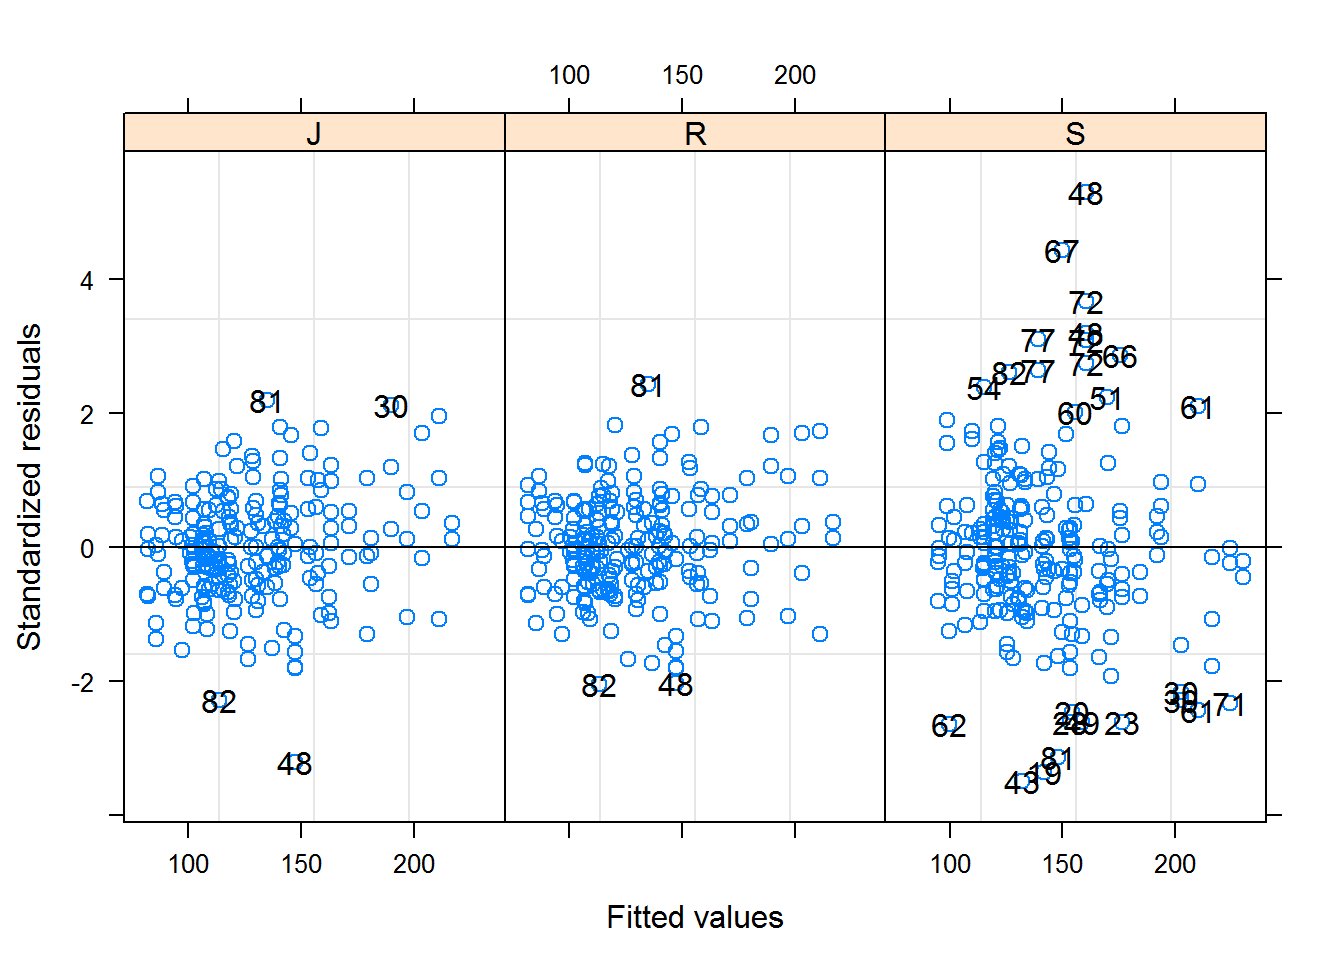
\includegraphics[width=0.9\linewidth]{images/bloodnlmeResidPlot2}
%		\caption{}
%		\label{fig:blood}
%	\end{figure}





\begin{framed}
	\begin{verbatim}
	data.frame( response = resid(JS.ARoy20091, type = "response"), 
	pearson  = resid(JS.ARoy20091, type = "pearson"), 
	normalized = resid(JS.ARoy20091, type = "normalized") )
	\end{verbatim}
\end{framed}

\begin{verbatim}
response      pearson    normalized
1    -4.65805902 -0.761587227 -0.7615872269
2    -0.88701342 -0.145025661  0.0776238081
3    -5.16580898 -0.844603753 -0.8446037530
4     2.29041830  0.374480726  0.6450898404
5     7.87508366  1.287567009  1.2875670086
6    -6.57048659 -1.074266908 -1.5090772378
...........................................
\end{verbatim}
For the $J$ observations, the variance is 6.116252 whereas for the $S$ observations, the denominator is 9.118144. (with the expected ratio of  1.490806)


\begin{framed}
	\begin{verbatim}
	> pearson %>%
	+   as.numeric %>% 
	+   matrix(nrow=85) %>%
	+   round(4) 
	[,1]    [,2]    [,3]    [,4]    [,5]    [,6]
	[1,] -0.7616  0.2194  0.3829 -0.2983  0.3597 -0.0790
	[2,] -0.1450  0.1820 -0.1450 -0.5014  0.1567  0.2663
	[3,] -0.8446  0.4634  0.1364 -0.1630 -0.2727  0.1660
	[4,]  0.3745 -0.2795 -0.2795 -0.2658 -0.2658  0.6115
	[5,]  1.2876 -0.6744 -0.6744  0.8935 -0.0935 -0.8612
	[6,] -1.0743  1.8687 -0.7473 -0.0383  0.2908 -0.3673
	...........................................
	
	\end{verbatim}
\end{framed}

We can plot the residuals against the fitted values, to assess the assumption of constant variance. 
\begin{framed}
	\begin{verbatim}
	# standardized residuals versus fitted values 
	plot(JS.ARoy20091, resid(., type = "pearson") ~ fitted(.) , 
	abline = 0, id = 0.05)
	\end{verbatim}
\end{framed}


\begin{framed}
	\begin{verbatim}
	par(mfrow=c(1,2))
	qqnorm((resid(JS.ARoy20091)[1:255]),
	pch="*",col="red",
	ylim=c(-40,40),
	main="Method J")
	qqline(resid(JS.ARoy20091)[1:255],col="blue")
	qqnorm((resid(JS.ARoy20091)[256:510]),
	pch="*",col="red",
	ylim=c(-40,40),
	main="Method S")
	qqline(resid(JS.ARoy20091)[256:510],col="blue")
	par(mfrow=c(1,1))
	\end{verbatim}	
\end{framed}

This code will allow you to make QQ plots for each level of the random effects.  LME models assume that not only the within-cluster residuals are normally distributed, but that each level of the random effects are as well. Depending on the model, you can vary the level from 0, 1, 2 and so on
\begin{framed}
	\begin{verbatim}
	qqnorm(JS.ARoy20091, ~ranef(.))
	
	# 	qqnorm(JS.ARoy20091, ~ranef(.,levels=1)
	\end{verbatim}
\end{framed}
\begin{figure}[h!]
	\centering
	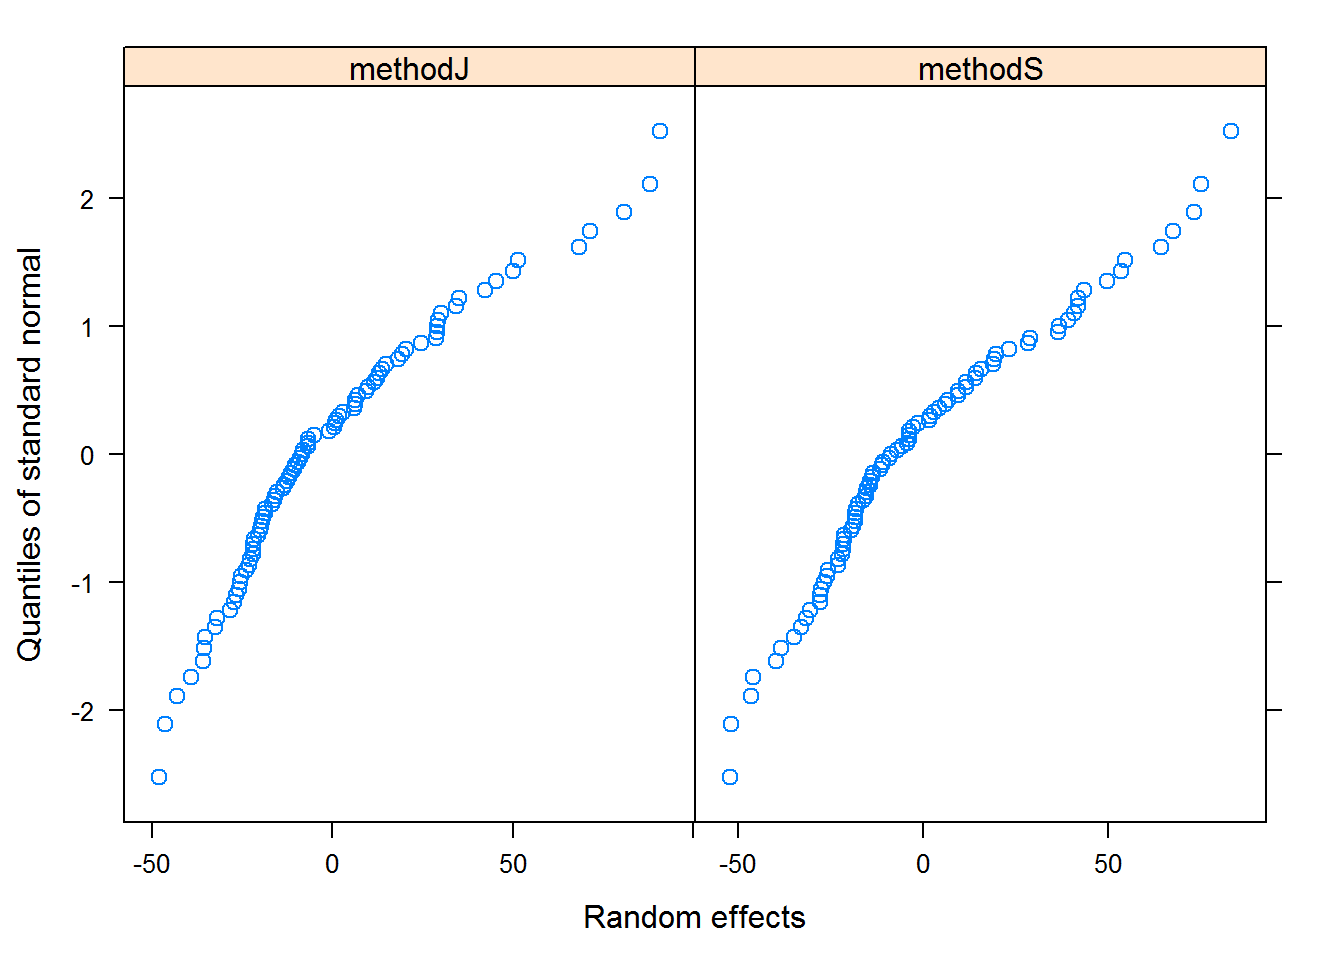
\includegraphics[width=0.9\linewidth]{images/ResidPlot2}
	\caption{}
	\label{fig:ResidPlot2}
\end{figure}	


\begin{framed}
	\begin{verbatim}
	data.frame( response = resid(JS.roy1, type = "response"), 
	pearson  = resid(JS.roy1, type = "pearson"), 
	normalized = resid(JS.roy1, type = "normalized") )
	\end{verbatim}
\end{framed}

\begin{verbatim}
response      pearson    normalized
1    -4.65805902 -0.761587227 -0.7615872269
2    -0.88701342 -0.145025661  0.0776238081
3    -5.16580898 -0.844603753 -0.8446037530
4     2.29041830  0.374480726  0.6450898404
5     7.87508366  1.287567009  1.2875670086
6    -6.57048659 -1.074266908 -1.5090772378
...........................................
\end{verbatim}
For the $J$ observations, the variance is 6.116252 whereas for the $S$ observations, the denominator is 9.118144. (with the expected ratio of  1.490806)


\begin{framed}
	\begin{verbatim}
	> pearson %>%
	+   as.numeric %>% 
	+   matrix(nrow=85) %>%
	+   round(4) 
	[,1]    [,2]    [,3]    [,4]    [,5]    [,6]
	[1,] -0.7616  0.2194  0.3829 -0.2983  0.3597 -0.0790
	[2,] -0.1450  0.1820 -0.1450 -0.5014  0.1567  0.2663
	[3,] -0.8446  0.4634  0.1364 -0.1630 -0.2727  0.1660
	[4,]  0.3745 -0.2795 -0.2795 -0.2658 -0.2658  0.6115
	[5,]  1.2876 -0.6744 -0.6744  0.8935 -0.0935 -0.8612
	[6,] -1.0743  1.8687 -0.7473 -0.0383  0.2908 -0.3673
	...........................................
	
	\end{verbatim}
\end{framed}

We can plot the residuals against the fitted values, to assess the assumption of constant variance. 
\begin{framed}
	\begin{verbatim}
	# standardized residuals versus fitted values 
	plot(JS.roy1, resid(., type = "pearson") ~ fitted(.) , 
	abline = 0, id = 0.05)
	\end{verbatim}
\end{framed}
\begin{figure}[h!]
	\centering
	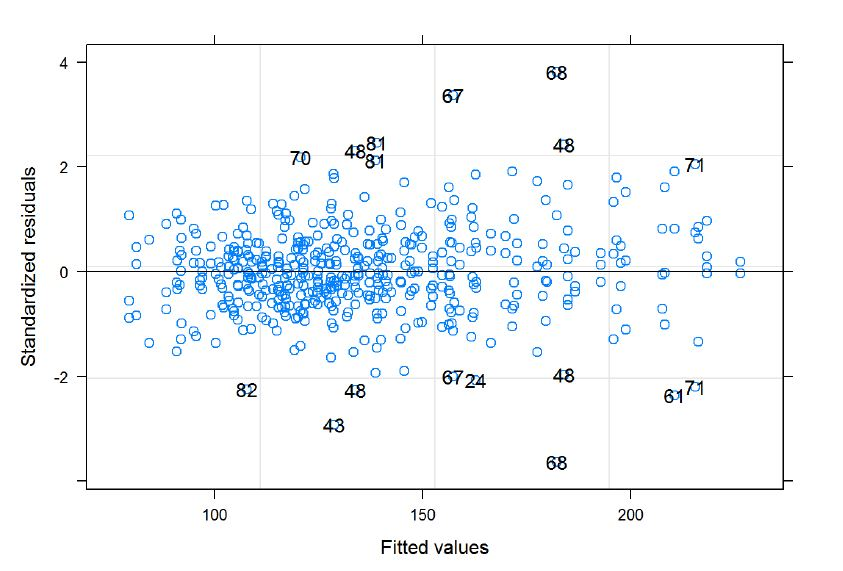
\includegraphics[width=0.9\linewidth]{images/Residuals-JS-Roy}
	\caption{}
	\label{fig:Residuals-JS-Roy}
\end{figure}


\begin{itemize}
	\item
	The \textbf{Scale-Location} plot, also called ‘Spread-Location’ or ‘S-L’ plot, takes the square root of the absolute residuals in order to diminish skewness (sqrt(|E|)) is much less skewed than | E | for Gaussian zero-mean E).
	
	\item
	The \textbf{Residual-Leverage} plot shows contours of equal Cook's distance, for values of cook.levels (by default 0.5 and 1) and omits cases with leverage one with a warning. If the leverages are constant (as is typically the case in a balanced aov situation) the plot uses factor level combinations instead of the leverages for the x-axis. (The factor levels are ordered by mean fitted value.)
\end{itemize}
%\begin{framed}
	\begin{verbatim}
	par(mfrow=c(4,1))
	plot(fittedmodel)
	par(opar)
	\end{verbatim}
%\end{framed}

%---------------------------------------------------------------------------%

\subsection{Residual Plots}
A residual plot is a graph that shows the residuals on the vertical axis and the independent variable on the horizontal axis. If the points in a residual plot are randomly dispersed around the horizontal axis, a linear regression model is appropriate for the data; otherwise, a non-linear model is more appropriate.

Below the table on the left shows inputs and outputs from a simple linear regression analysis, and the chart on the right displays the residual (e) and independent variable (X) as a residual plot.

\begin{verbatim}
x &	60	& 70	& 80	& 85 &	95 \\ \hline
y &	70	& 65	& 70	& 95 &	85 \\ \hline
y.hat	65.411	71.849	78.288	81.507	87.945
e	4.589	-6.849	-8.288	13.493	-2.945
\end{verbatim}


The residual plot shows a fairly random pattern - the first residual is positive, the next two are negative, the fourth is positive, and the last residual is negative. This random pattern indicates that a linear model provides a decent fit to the data.

Below, the residual plots show three typical patterns. The first plot shows a random pattern, indicating a good fit for a linear model. The other plot patterns are non-random (U-shaped and inverted U), suggesting a better fit for a non-linear model.




\bibliography{DB-txfrbib}
\end{document}